% =============================================================================
% sections/design/rover/software_overview.tex  -  Software Overview
% Teams: electronics / navigation (best guess - unconfirmed) / Status: EXAMPLE (scope approximation)
%
% EXAMPLE CONTENT for scope/layout approximation - not final report text.
% Adapted from the Preliminary Report's "Software Architecture" intro,
% trimmed to minimal prose. Marked with \exampleflag on its heading in the
% assembler.
%
% Image is a placeholder (figures/software_architecture.png) - swap it for
% the real ROS 2 node graph by overwriting the same file. Shared figures/
% (not a team folder) since this is a whole-rover, system-level diagram.
% =============================================================================

The rover's software stack is built on ROS 2 Humble as the middleware
framework, providing standardized inter-process communication via topics,
services, and actions, and integrating with the broader ROS 2 ecosystem of
navigation, perception, and control packages used throughout the system.
\autoref{fig:software_architecture} shows the resulting node-level
architecture.

\begin{figure}[!htbp]
    \centering
    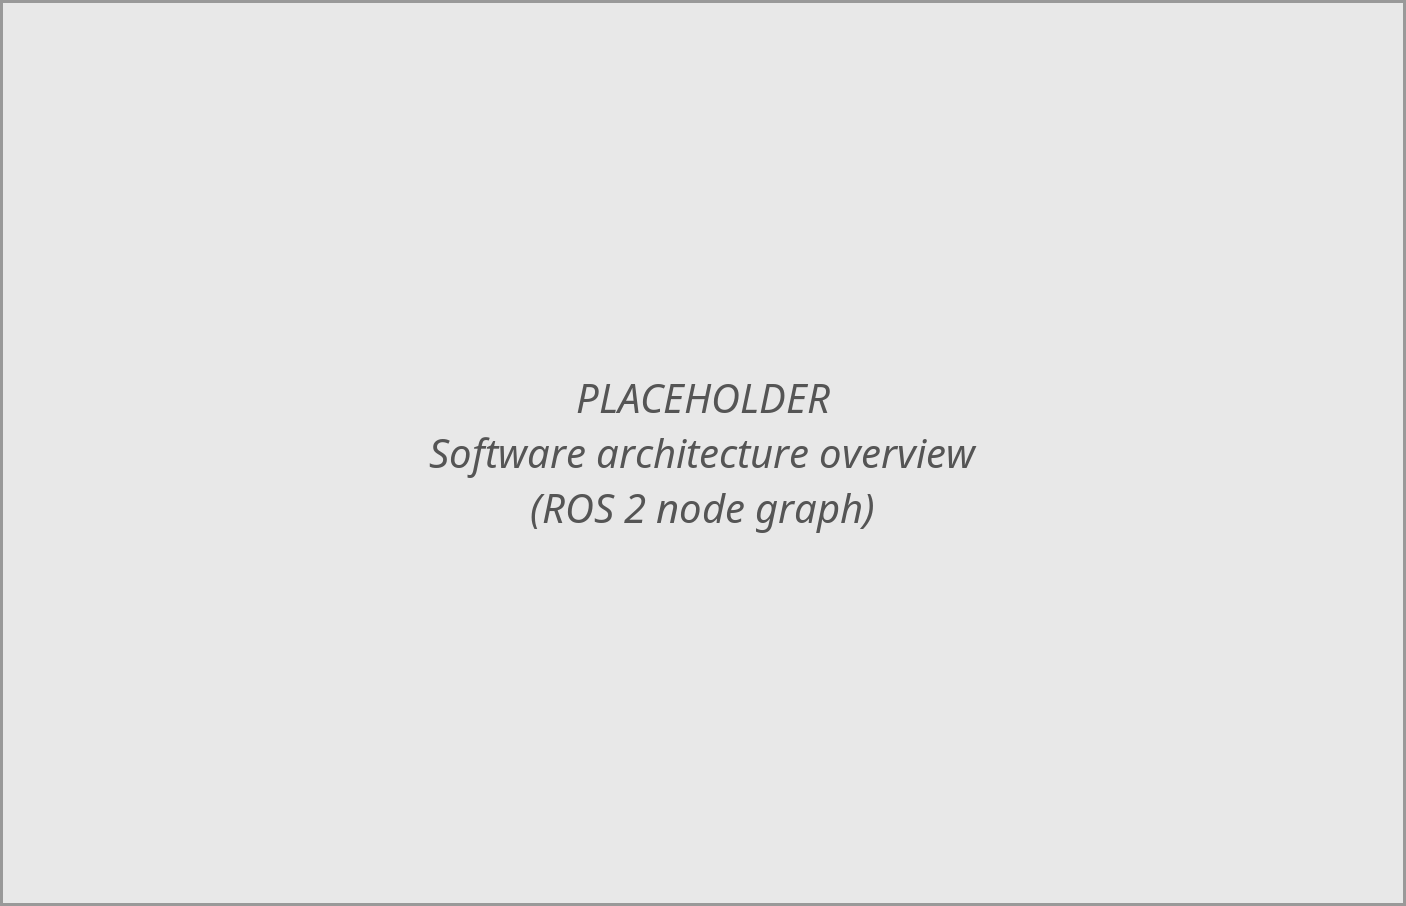
\includegraphics[width=0.85\linewidth]{figures/software_architecture}
    \caption{Software architecture overview}
    \label{fig:software_architecture}
\end{figure}
